\subsection{Benchmark UPPAAL}\label{sub:benchmark_uppaal}
More states should intuitively mean UPPAAL runs slower, however this might not be the case if these extra states are easily pruneable.
Therefore we tried running the same query twice in UPPAAL on a large timed word.
The timed word used in these examples are 34198 timed characters long, and the last character happens at time 238817.
The data of these benchmarks can be found on \cref{table:uppaal_benchmarks}.

\begin{tabular}{|c|c|c|c|c|}
    \hline
    & States & Edges & Clocks & Time \\
    \hline
    Pruning & 6 & 8 & 3 & 76s \\
    \hline
    No pruning & 10 & 12 & 3 & 103s \\
    \hline
\end{tabular}
\captionof{table}{Table of benchmarks in UPPAAL.}
\label[table]{table:uppaal_benchmarks}

As can be seen on \cref{table:uppaal_benchmarks}, checking is faster with pruning.
This points to UPPAAL not pruning the unnecessary states when checking.
So pruning not only helps with readability, it also helps with performance. 

\subsection{Benchmark TREAT}
\subsubsection{Setup}
Next step is checking if the prunings have an effect on performance on TREAT.
The original implementation pruned steps after generating the entire automaton.
However, it might be faster if pruning is performed while generating the automaton.
For this reason, we have created a series of regular expressions and test configurations, and put them all against each other to see how each perform.
Each configuration is a mix of pruning before and after generation of the automaton.

\begin{enumerate}
    \item \textbf{N}: This configuration has no pruning.
    \item \textbf{S}: This configuration prunes only states after generation.
    \item \textbf{E}: This configuration prunes everything after generation.
    \item \textbf{SS}: This configuration prunes states during generation and everything after generation.
    \item \textbf{SE}: This configuration prunes states during generation and only states after generation.
    \item \textbf{ES}: This configuration prunes everything during generation and only states after generation.
    \item \textbf{EE}: This configuration prunes everything during generation and everything after generation.
\end{enumerate}

Note: When we say prune during generation, we are talking about pruning the operands of the explosive operators.
This means the left and right operand of an intersection and the single operand of an absorbed iterator.

As for the tests we have generated 6 parameterized TREs, that we use to generate a total of 19 unique TREs.
Each TRE serves a unique purpose.
All these TREs can be found in \cref{app:RegularExpressionTable}.

TREs $a$, $b$ and $f$ were all chosen because they would benefit from pruning while generating.
, serving as a best case scenario for SS, SE, ES and EE.
The theory being, that these configurations limit the amount of states used in the explosive operators, therefore making them less explosive.
Ideally it should make them resemble a linear complexity, since the final TAs are of constant length.

TRE $c$, $d$ and $e$ where all chosen to benefit no pruning while generating.
, serving as a best case scenario for N, S and E.
The theory being these regular expressions wont benefit from pruning while generating, since a limited or no pruning can be done during generation.

\subsubsection{Results}
The results can be split into 3 main categories.

\begin{enumerate}
    \item Equivalent performance between configurations.
    \item SS, SE, ES and EE configurations are better.
    \item N, S, SS configurations are better.
\end{enumerate}

All the plots can be seen on \cref{sec:BenchmarkGraphs}, with all the data on \cref{sec:BenchmarkTable}, however a few will be presented here.

The TREs $a$, $b$, $d$ and $e$ are all equivalent in performance.
By this we mean their graphs are all curved in the same way, and they are within a few percentages of each other.
An example of this can be seen on \cref{fig:mean3-5} (this is the one with the biggest difference in this category).

\resizebox{\columnwidth}{!}{
    % 3,4,5
\plot{1,2,4}
{(1,5352.0)(2,33275.6)(4,14345441.6)}
{(1,7892.0)(2,46225.8)(4,21889111.1)}
{(1,6849.0)(2,39386.9)(4,15581794.2)}
{(1,5774.6)(2,18779.8)(4,6445558.3)}
{(1,6492.7)(2,21796.9)(4,9163154.7)}
{(1,6098.4)(2,17999.6)(4,3569375.9)}
{(1,6843.2)(2,20351.3)(4,5761799.7)}
}

\resizebox{\columnwidth}{!}{
    % 3,4,5
\plot{1,2,4}
{(1,5352.0)(2,33275.6)(4,14345441.6)}
{(1,7892.0)(2,46225.8)(4,21889111.1)}
{(1,6849.0)(2,39386.9)(4,15581794.2)}
{(1,5774.6)(2,18779.8)(4,6445558.3)}
{(1,6492.7)(2,21796.9)(4,9163154.7)}
{(1,6098.4)(2,17999.6)(4,3569375.9)}
{(1,6843.2)(2,20351.3)(4,5761799.7)}
}
\captionof{figure}{Graphs for time and memory of regular expression 3-5 ($b$).}
\label{fig:mean3-5}

Since we were expecting $a$ and $b$ to be more performant on SS, SE, ES and EE, this result is not what we expected.
After opening up one of the automata (\cref{fig:FailedAutomata}) we can see state $q1$ should have been pruned, since it can never be reached from the starting state.
However it is not pruned, because it is neither unreachable nor dead because of the self loop.
So we have a problem where a loop to a state itself will keep a state throughout our pruning rules.

% File Generated Automatically
%
% NOTICE: This file has been generated automatically.
% Any manual modifications made to this file may be
% overwritten the next time it is generated.
%
% Generated by: TimedRegex, Version = 1.0.0.0
% Date 5/24/2024 10:27:37 AM
\usetikzlibrary {automata,positioning}
% "((J)+')+'"
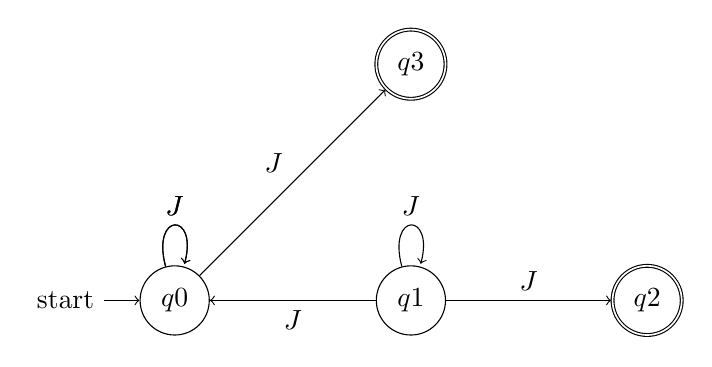
\begin{tikzpicture}[auto]
    \node[state, initial] at (6, 0)(q0){$q0$};
    \node[state] at (9, 0)(q1){$q1$};
    \node[state, accepting] at (12, 0)(q2){$q2$};
    \node[state, accepting] at (9, 3)(q3){$q3$};
    
    \path[->]
        (q1)edge node{$J$}(q2)
        (q1)edge node{$J$}(q0)
        (q0)edge node{$J$}(q3)
        (q0)edge [loop above] node{$J$}(q0)
        (q1)edge [loop above] node{$J$}(q1)
        (q0)edge [loop above] node{$J$}(q0)
        ;
\end{tikzpicture}
 


Creating bigger automata only expands on this problem. This is something that could be fixed, but for now we are leaving it as is.

The TRE $f$ performs better on SS, SE, ES and EE.
This graph can be seen on \cref{fig:mean15-19}.
This is the kind of performance difference we expected, and proves pruning while generation is a lot better for intersection.

\resizebox{\columnwidth}{!}{
    % 15,16,17,18,19
\plotmem{1,2,4,8,16}
{(1,2.38) (2,12.3)(4,59.38)(8,917.55)   (16,315469.2)}
{(1,4.75)(2,15.5)(4,83.24)(8,2515.32)  (16,1955655.8)}
{(1,3.73)(2,13.86)(4,62.1)(8,934.43)   (16,321366.52)}
{(1,3.73)(2,13.37)(4,33.36)(8,76.75)    (16,174.71)}
{(1,4.75)(2,14.63)(4,36.13)(8,86.02)    (16,208.98)}
{(1,3.73)(2,15.4)(4,39.59)(8,89.39)    (16,193.98)}
{(1,4.75)(2,16.66)(4,40.86)(8,90.66)    (16,195.24)}
}

\resizebox{\columnwidth}{!}{
    % 15,16,17,18,19
\plotmem{1,2,4,8,16}
{(1,2.38) (2,12.3)(4,59.38)(8,917.55)   (16,315469.2)}
{(1,4.75)(2,15.5)(4,83.24)(8,2515.32)  (16,1955655.8)}
{(1,3.73)(2,13.86)(4,62.1)(8,934.43)   (16,321366.52)}
{(1,3.73)(2,13.37)(4,33.36)(8,76.75)    (16,174.71)}
{(1,4.75)(2,14.63)(4,36.13)(8,86.02)    (16,208.98)}
{(1,3.73)(2,15.4)(4,39.59)(8,89.39)    (16,193.98)}
{(1,4.75)(2,16.66)(4,40.86)(8,90.66)    (16,195.24)}
}
\captionof{figure}{Graphs for time and memory of regular expression 15-19 ($f$).}
\label{fig:mean15-19}

Finally the TRE $c$ performs better on N, S and SS.
This graph can be seen on \cref{fig:mean6-8}
This is probably because the pruning of everything is too expensive in terms of time and memory for it to make sense for this automaton.
While this is an interesting result, it does not mean these prunings are better, since they dont get rid of all the extra states.

\resizebox{\columnwidth}{!}{
    % 6,7,8
\plotmem{64,128,256}
{(64,2774.94)    (128,9617.03)     (256,36055.38)}
{(64,158752.09)  (128,1245220.51)  (256,9871874.21)}
{(64,2799.35)    (128,9667.24)     (256,36160.29)}
{(64,2338.61)    (128,8618.71)     (256,33125.43)}
{(64,14810.97)   (128,102171.73)  (256,756806.44)}
{(64,112051.15)  (128,884427.52)  (256,7031719.82)}
{(64,124523.45)  (128,977979.83)  (256,7755400.13)}
}

\resizebox{\columnwidth}{!}{
    % 6,7,8
\plotmem{64,128,256}
{(64,2774.94)    (128,9617.03)     (256,36055.38)}
{(64,158752.09)  (128,1245220.51)  (256,9871874.21)}
{(64,2799.35)    (128,9667.24)     (256,36160.29)}
{(64,2338.61)    (128,8618.71)     (256,33125.43)}
{(64,14810.97)   (128,102171.73)  (256,756806.44)}
{(64,112051.15)  (128,884427.52)  (256,7031719.82)}
{(64,124523.45)  (128,977979.83)  (256,7755400.13)}
}
\captionof{figure}{Graphs for time and memory of regular expression 6-8 ($c$).}
\label{fig:mean6-8}

\subsubsection{Conclusions}
We have shown that in UPPAAL you can gain significant performance by pruning the states.
, so pruning should be worth it to do most of the time, since pruning is a startup cost.

Pruning by itself can lead to really explosive performance on some regular expressions.
, even if we prune while the automaton is generating.
However, in the large picture, it seems like pruning during generation has the ability to turn some generations from parabolic to linear.
